%!TEX root = ../draft.tex

\begin{appendices}
% \adjustmtc 
\renewcommand{\appendixname}{ANHANG}
\renewcommand{\appendixtocname}{\appendixname} 
\addappheadtotoc 

% \begin{mtchideinmaintoc}[0]   %  [-1] Den folgenden Inhalt nicht im großen Inhaltsverzeichnis zeigen, [0] ab Chapter im großen Inhaltsverzeichnis anzeigen

\part*{Anhang}
\begin{figure}[htb]
\begin{minipage}[c]{0.2\textwidth}
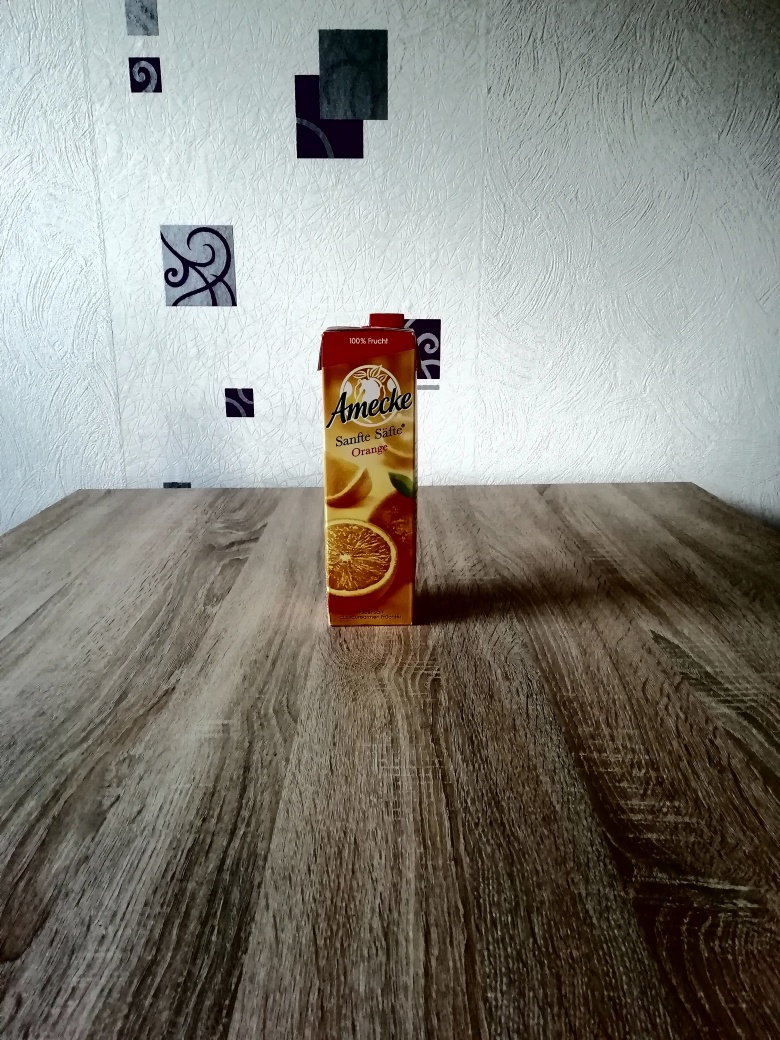
\includegraphics[width=\textwidth]{Sources/Bild1_HA.jpg}
\end{minipage}
\hfill
\begin{minipage}[c]{0.08\textwidth}
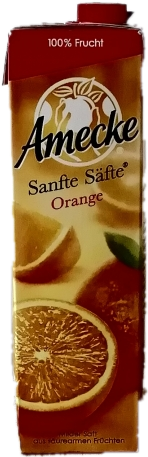
\includegraphics[width=\textwidth]{Sources/Bild1_HA.png}
\end{minipage}
\hfill
\begin{minipage}[c]{0.3\textwidth}
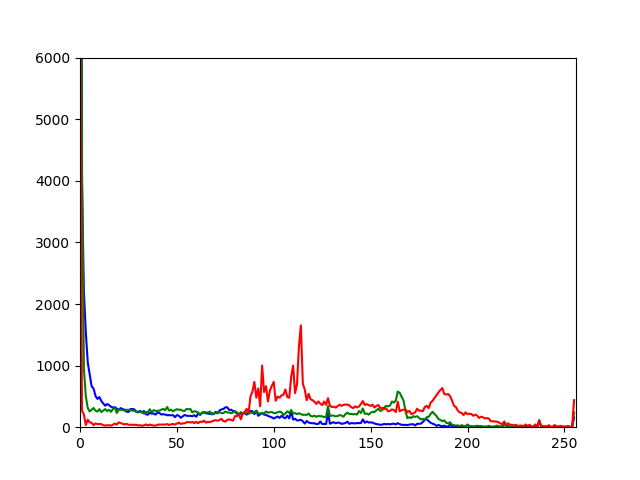
\includegraphics[width=\textwidth]{Sources/Bild1_HA_histo.png}
\end{minipage}
\end{figure}
\begin{figure}[htb]
\begin{minipage}[c]{0.2\textwidth}
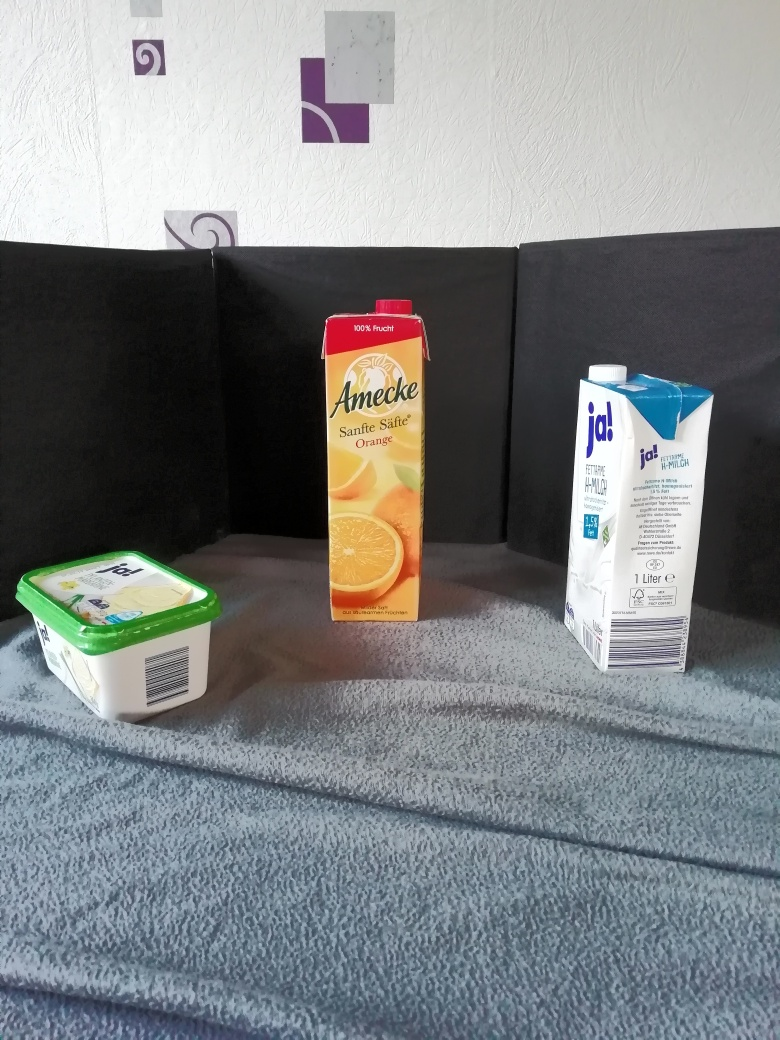
\includegraphics[width=\textwidth]{Sources/Bild2_HA.jpg}
\end{minipage}
\hfill
\begin{minipage}[c]{0.08\textwidth}
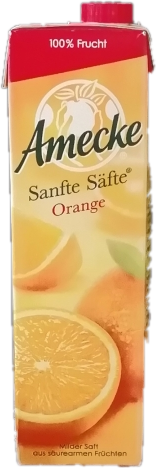
\includegraphics[width=\textwidth]{Sources/Bild2_HA.png}
\end{minipage}
\hfill
\begin{minipage}[c]{0.3\textwidth}
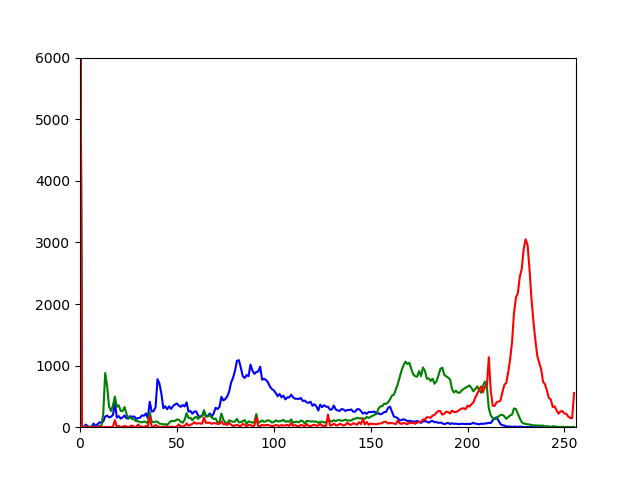
\includegraphics[width=\textwidth]{Sources/Bild2_HA_histo.png}
\end{minipage}
\end{figure}
\begin{figure}[htb]
\begin{minipage}[c]{0.2\textwidth}
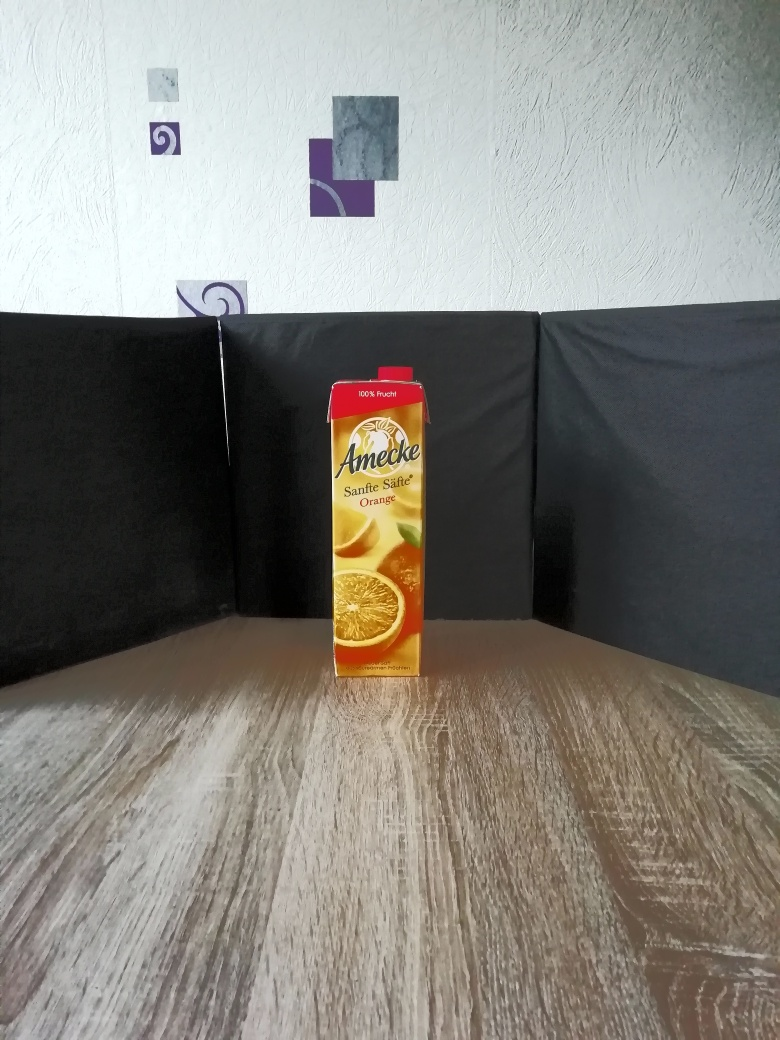
\includegraphics[width=\textwidth]{Sources/Bild3_HA.jpg}
\end{minipage}
\hfill
\begin{minipage}[c]{0.08\textwidth}
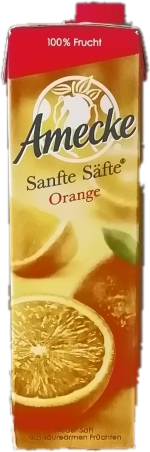
\includegraphics[width=\textwidth]{Sources/Bild3_HA.png}
\end{minipage}
\hfill
\begin{minipage}[c]{0.3\textwidth}
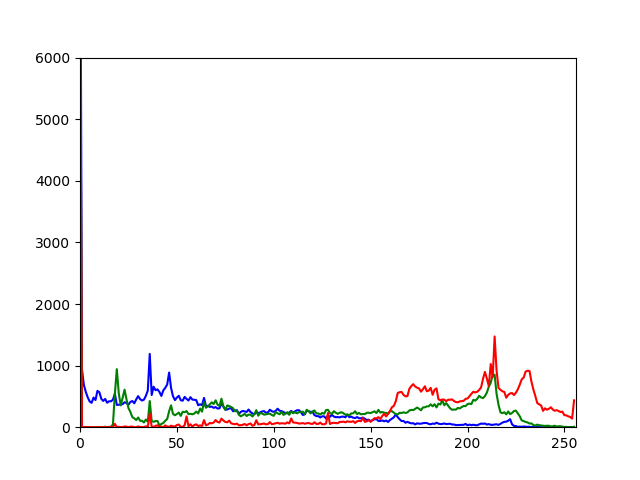
\includegraphics[width=\textwidth]{Sources/Bild3_HA_histo.png}
\end{minipage}
\caption{Histogramm des segmentierten Objektes aus dem Nahrungsmittel-Datensatz. Normalisiert durch den Histogramm-Ausgleich}
\label{img:evalHA}
\end{figure}
\newpage
\begin{figure}[htb]
\begin{minipage}[c]{0.2\textwidth}
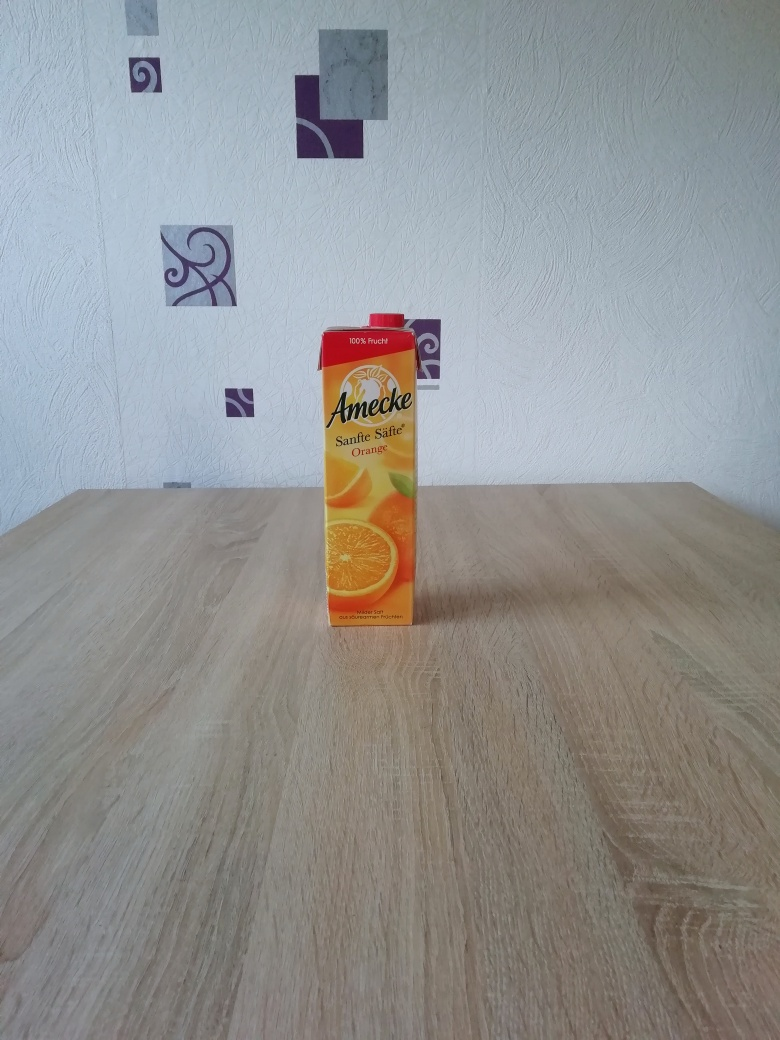
\includegraphics[width=\textwidth]{Sources/Bild1_GW.jpg}
\end{minipage}
\hfill
\begin{minipage}[c]{0.08\textwidth}
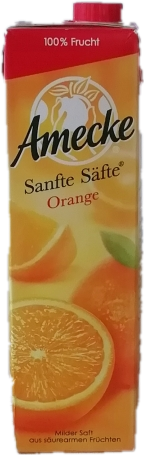
\includegraphics[width=\textwidth]{Sources/Bild1_GW.png}
\end{minipage}
\hfill
\begin{minipage}[c]{0.3\textwidth}
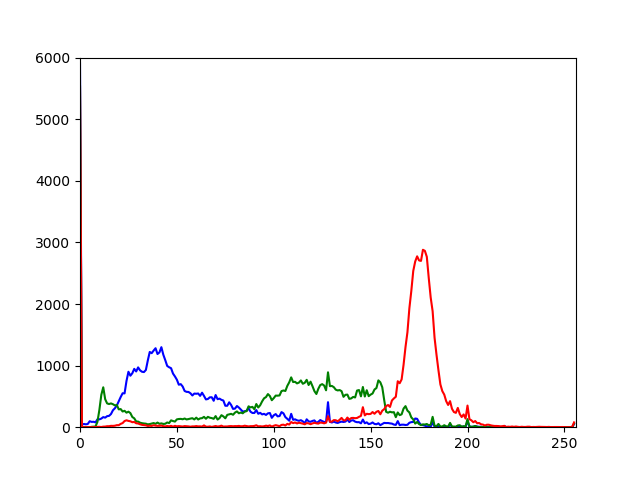
\includegraphics[width=\textwidth]{Sources/Bild1_GW_histo.png}
\end{minipage}
\end{figure}
\begin{figure}[htb]
\begin{minipage}[c]{0.2\textwidth}
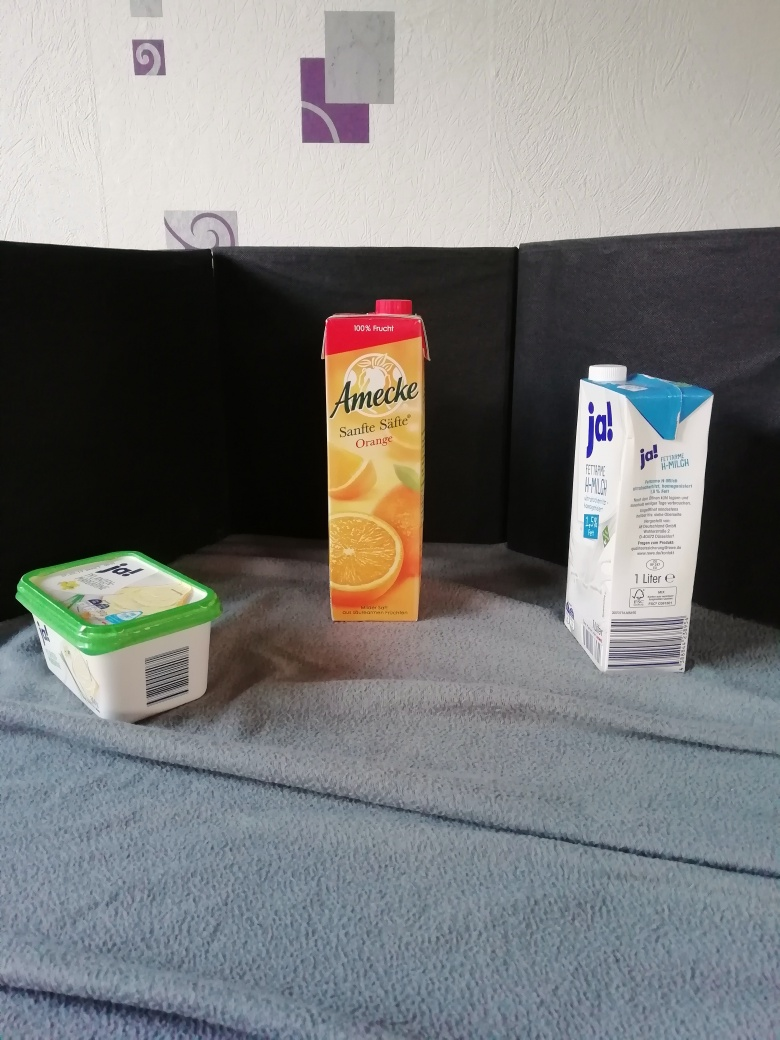
\includegraphics[width=\textwidth]{Sources/Bild2_GW.jpg}
\end{minipage}
\hfill
\begin{minipage}[c]{0.08\textwidth}
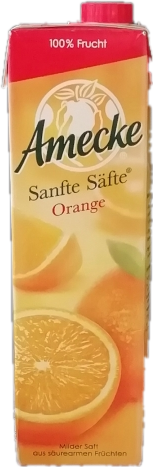
\includegraphics[width=\textwidth]{Sources/Bild2_GW.png}
\end{minipage}
\hfill
\begin{minipage}[c]{0.3\textwidth}
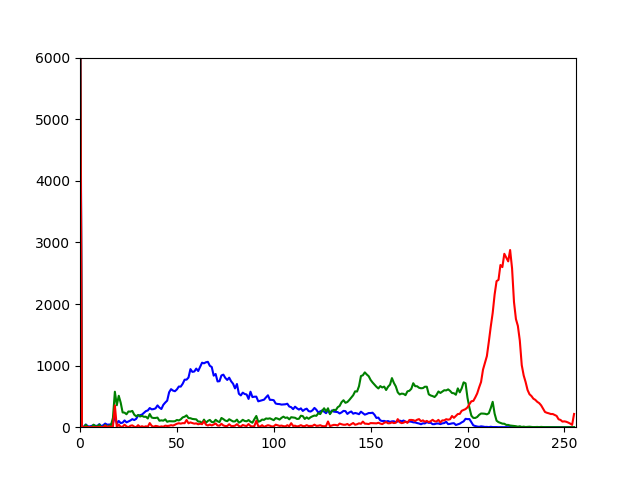
\includegraphics[width=\textwidth]{Sources/Bild2_GW_histo.png}
\end{minipage}
\end{figure}
\begin{figure}[htb]
\begin{minipage}[c]{0.2\textwidth}
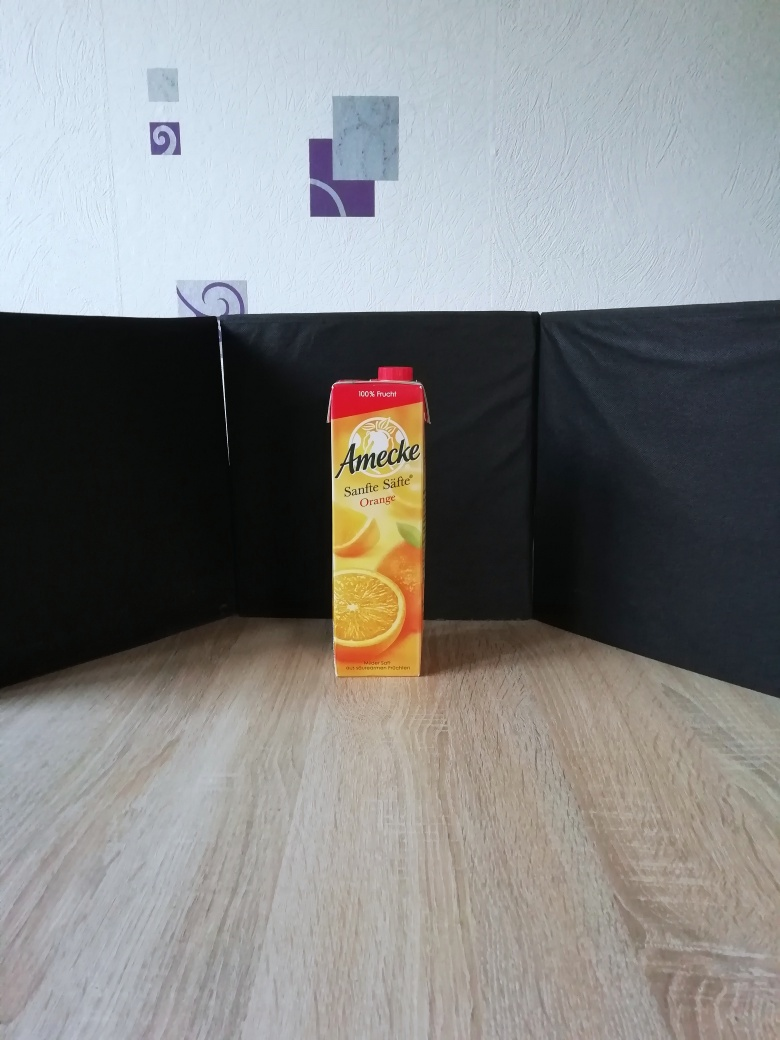
\includegraphics[width=\textwidth]{Sources/Bild3_GW.jpg}
\end{minipage}
\hfill
\begin{minipage}[c]{0.08\textwidth}
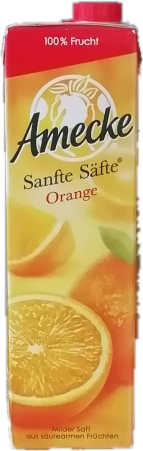
\includegraphics[width=\textwidth]{Sources/Bild3_GW.png}
\end{minipage}
\hfill
\begin{minipage}[c]{0.3\textwidth}
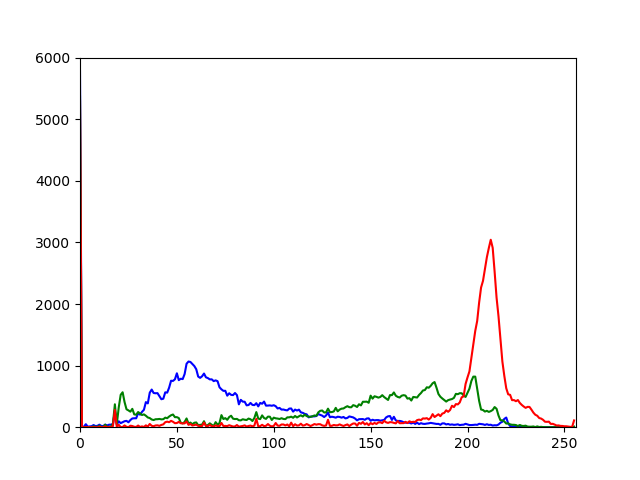
\includegraphics[width=\textwidth]{Sources/Bild3_GW_histo.png}
\end{minipage}
\caption{Histogramm des segmentierten Objektes aus dem Nahrungsmittel-Datensatz. Normalisiert durch den Gray-World-Algorithmus}
\label{img:evalGW}
\end{figure}
\newpage
\begin{figure}[htb]
\begin{minipage}[c]{0.2\textwidth}
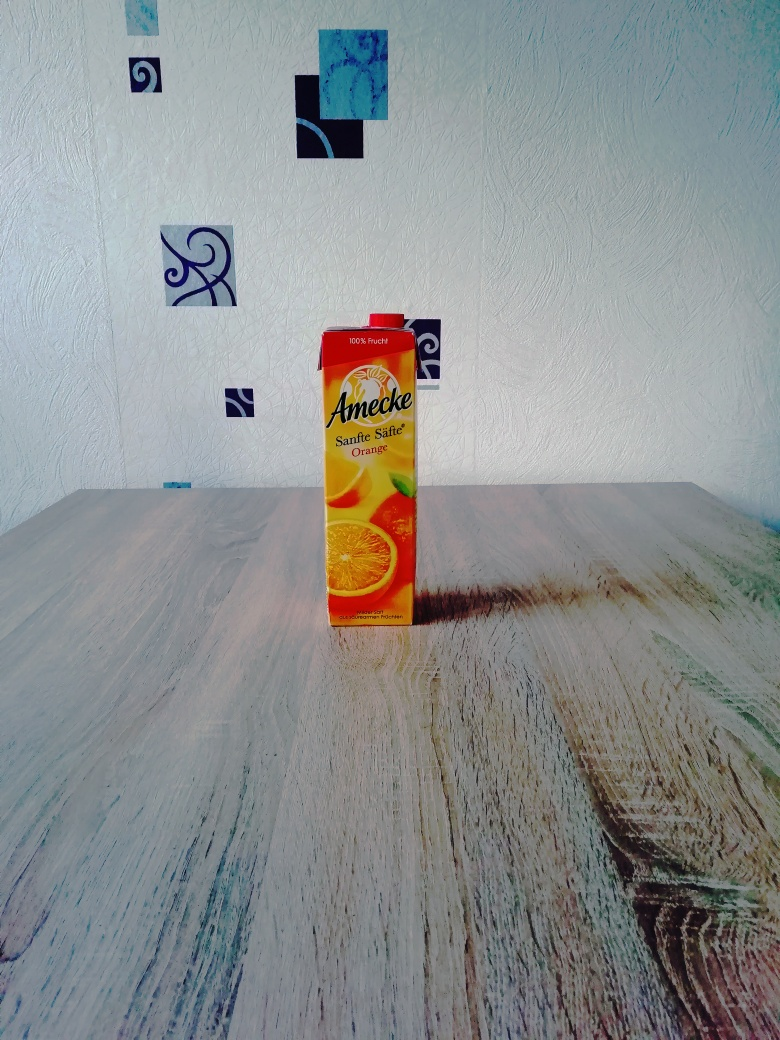
\includegraphics[width=\textwidth]{Sources/Bild1_HS.jpg}
\end{minipage}
\hfill
\begin{minipage}[c]{0.08\textwidth}
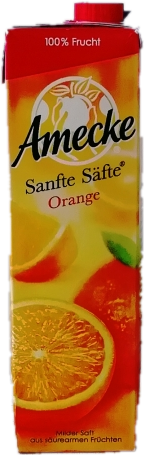
\includegraphics[width=\textwidth]{Sources/Bild1_HS.png}
\end{minipage}
\hfill
\begin{minipage}[c]{0.3\textwidth}
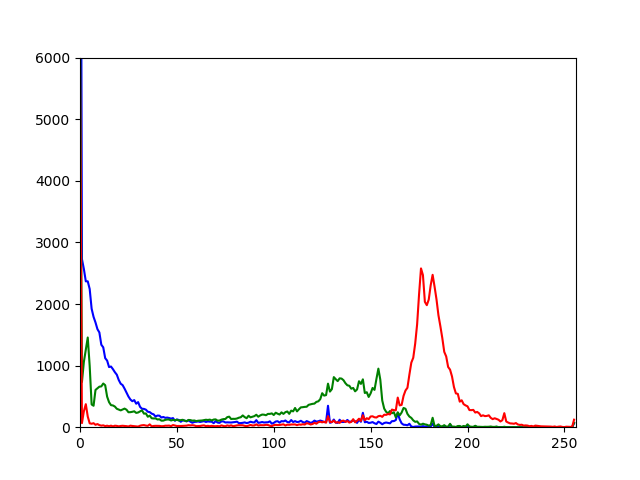
\includegraphics[width=\textwidth]{Sources/Bild1_HS_histo.png}
\end{minipage}
\end{figure}
\begin{figure}[htb]
\begin{minipage}[c]{0.2\textwidth}
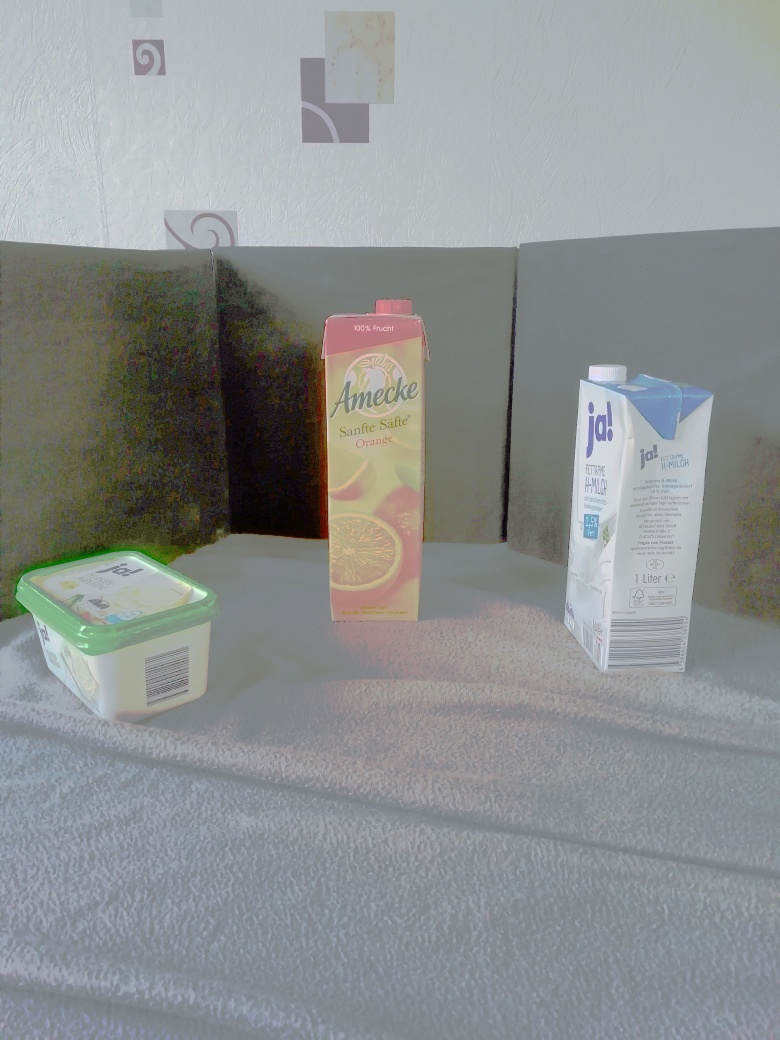
\includegraphics[width=\textwidth]{Sources/Bild2_HS.jpg}
\end{minipage}
\hfill
\begin{minipage}[c]{0.08\textwidth}
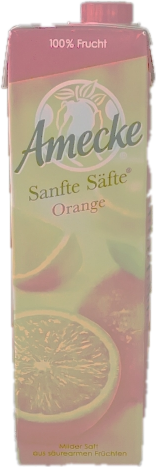
\includegraphics[width=\textwidth]{Sources/Bild2_HS.png}
\end{minipage}
\hfill
\begin{minipage}[c]{0.3\textwidth}
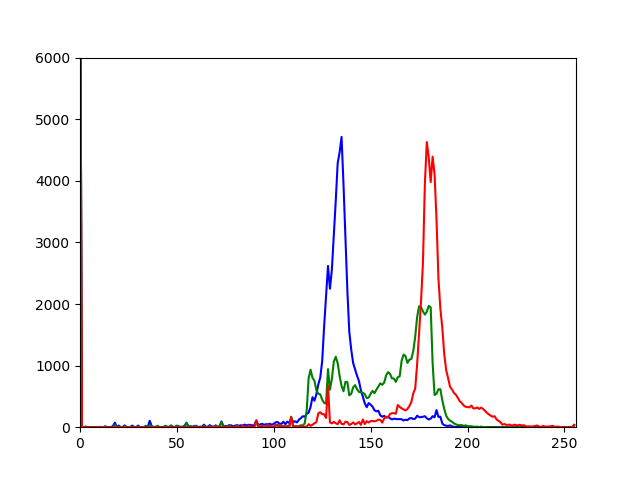
\includegraphics[width=\textwidth]{Sources/Bild2_HS_histo.png}
\end{minipage}
\end{figure}
\begin{figure}[htb]
\begin{minipage}[c]{0.2\textwidth}
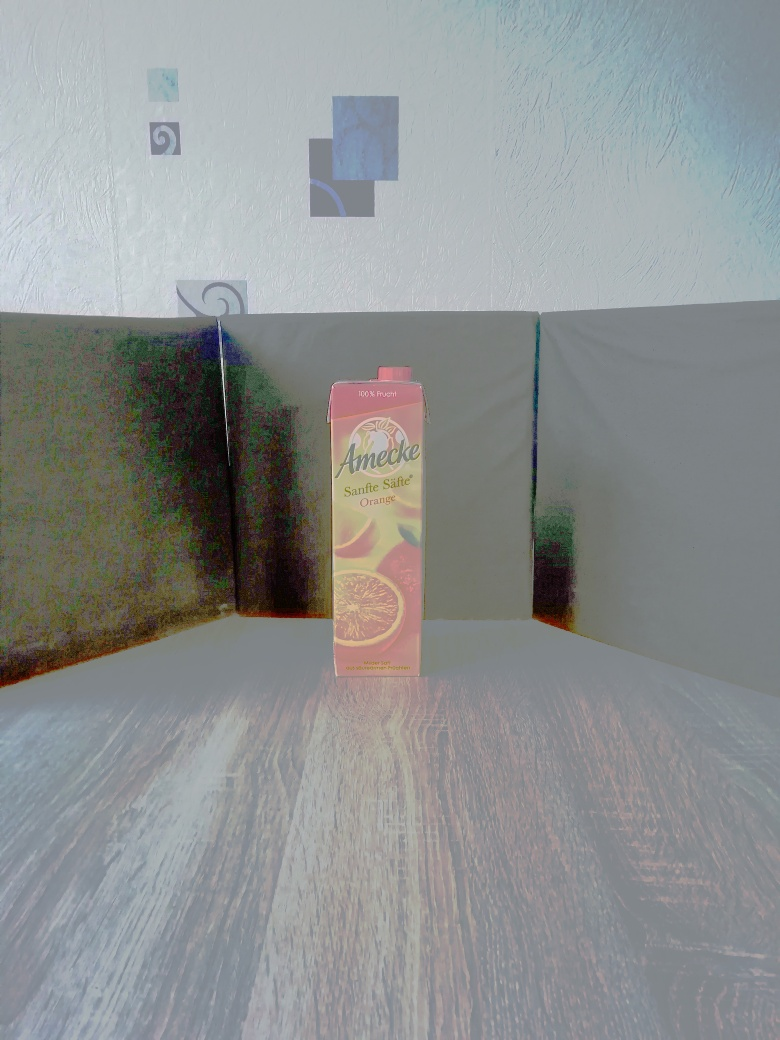
\includegraphics[width=\textwidth]{Sources/Bild3_HS.jpg}
\end{minipage}
\hfill
\begin{minipage}[c]{0.08\textwidth}
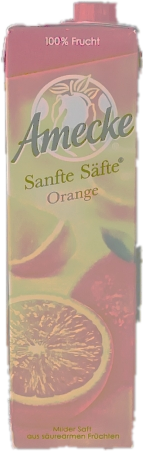
\includegraphics[width=\textwidth]{Sources/Bild3_HS.png}
\end{minipage}
\hfill
\begin{minipage}[c]{0.3\textwidth}
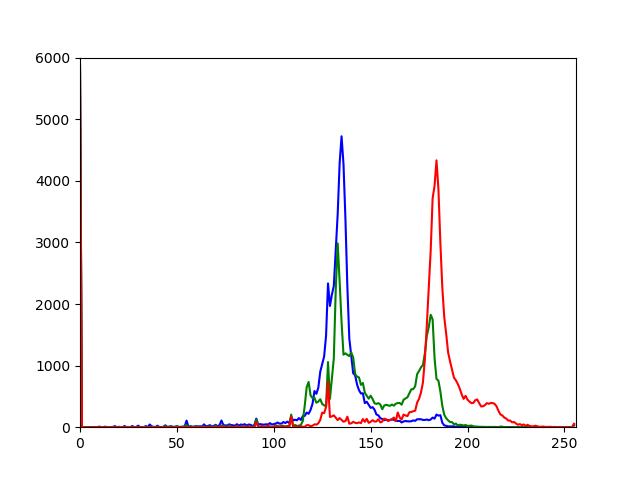
\includegraphics[width=\textwidth]{Sources/Bild3_HS_histo.png}
\end{minipage}
\caption{Histogramm des segmentierten Objektes aus dem Nahrungsmittel-Datensatz. Normalisiert durch die Histogramm-Spezifikation}
\label{img:evalHS}
\end{figure}
\begin{figure}[htbp]
\center
\begin{minipage}{0.49\textwidth}
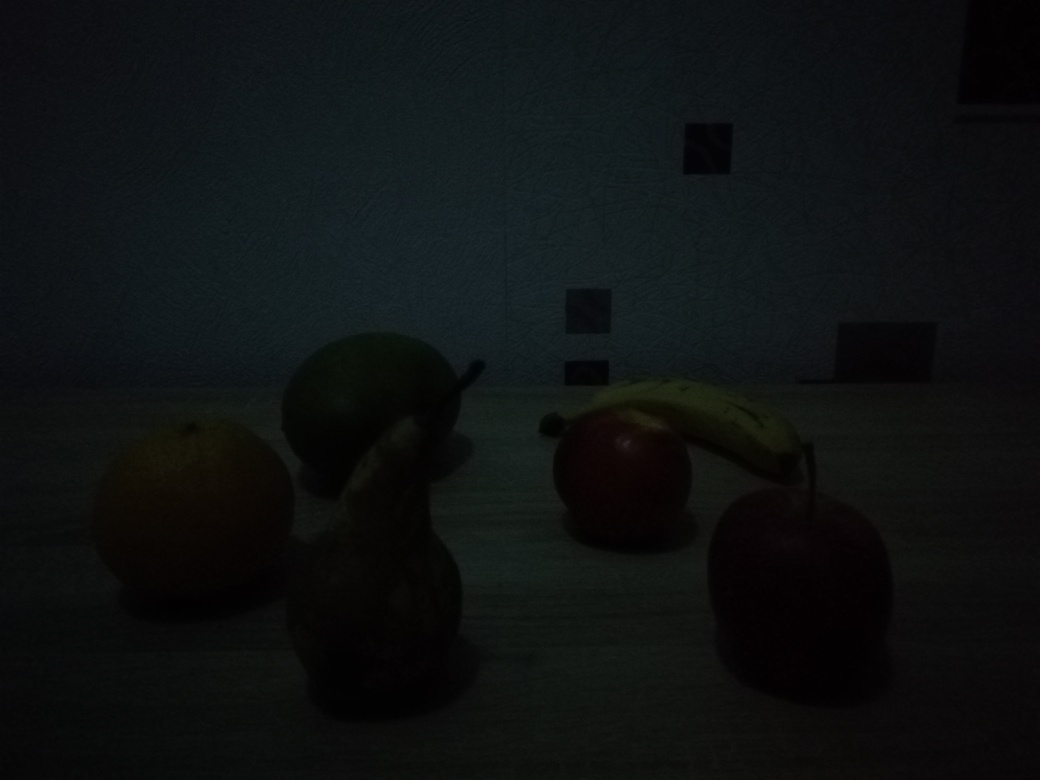
\includegraphics[width=.8\textwidth]{Sources/Anhang/resize_0250.jpg}
\end{minipage}
\begin{minipage}{0.49\textwidth}
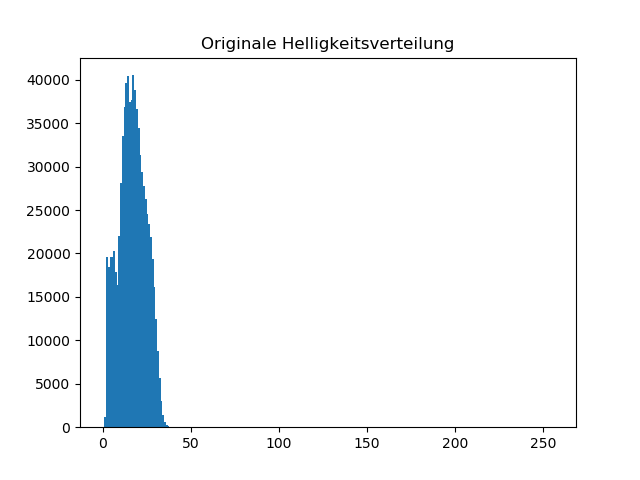
\includegraphics[width=\textwidth]{Sources/Anhang/resize_0250.png}
\end{minipage}
\begin{minipage}{0.49\textwidth}
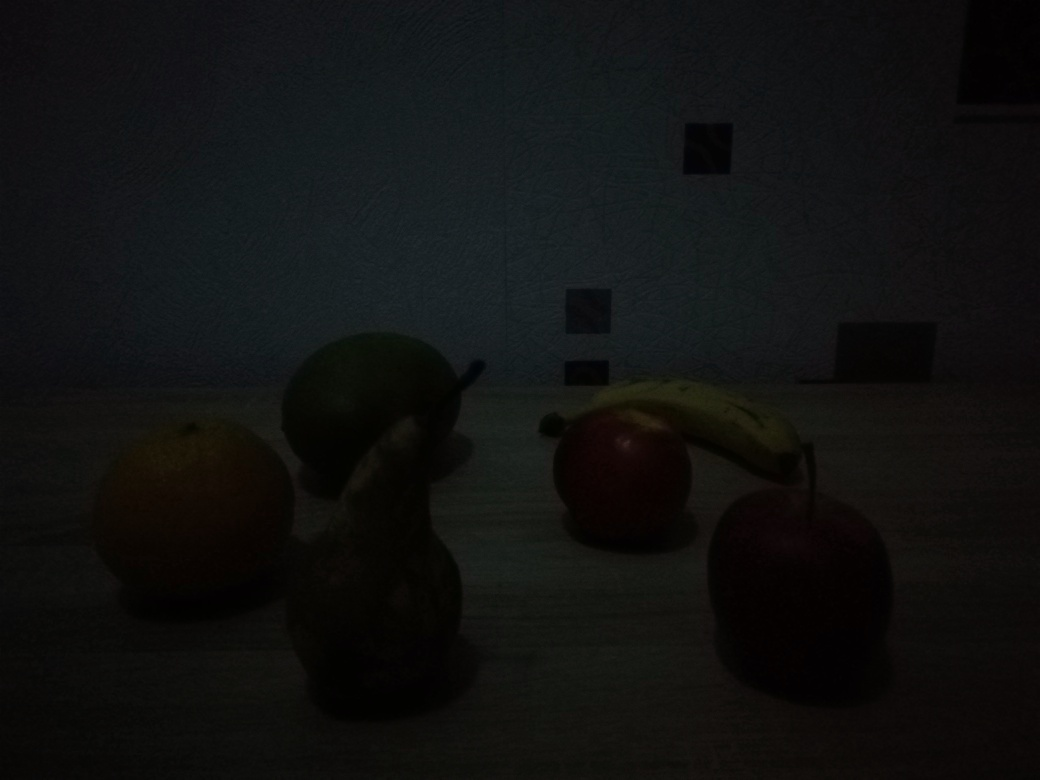
\includegraphics[width=.8\textwidth]{Sources/Anhang/resize_0250_GW.jpg}
\end{minipage}
\begin{minipage}{0.49\textwidth}
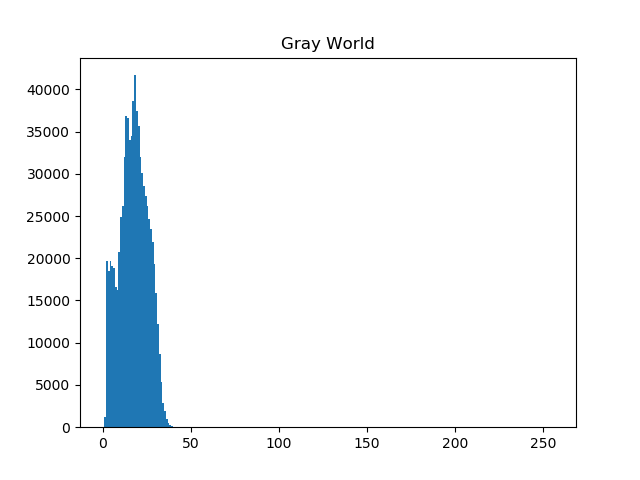
\includegraphics[width=\textwidth]{Sources/Anhang/resize_0250_GW.png}
\end{minipage}
\begin{minipage}{0.49\textwidth}
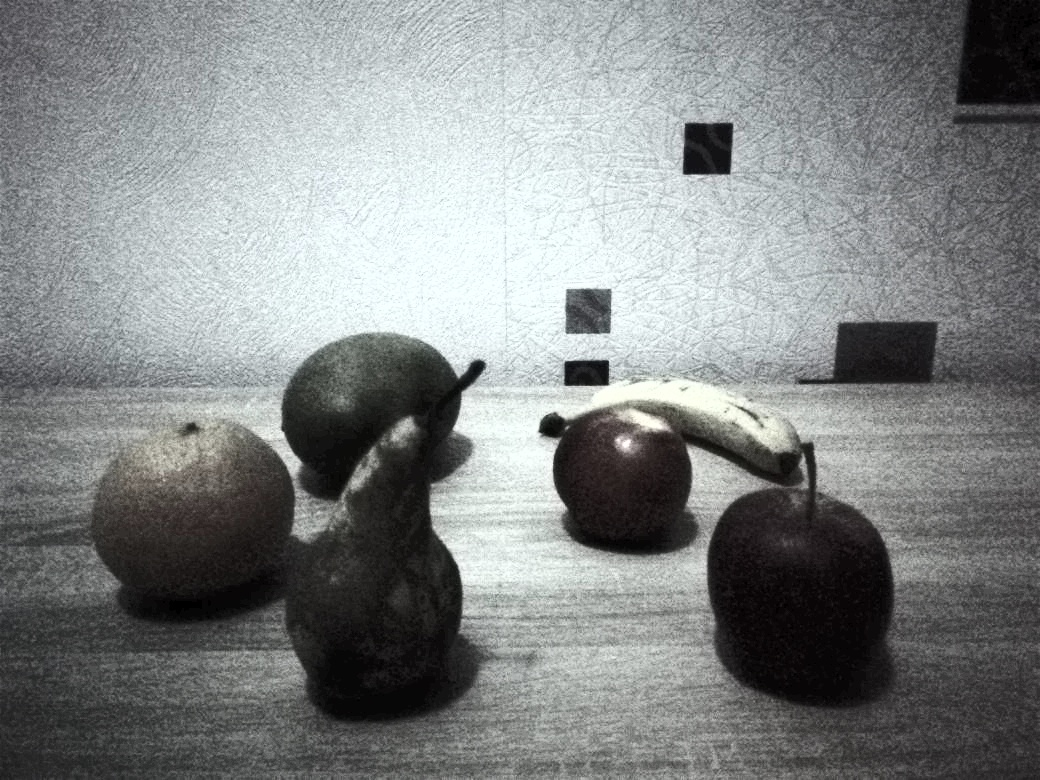
\includegraphics[width=.8\textwidth]{Sources/Anhang/resize_0250_HA.jpg}
\end{minipage}
\begin{minipage}{0.49\textwidth}
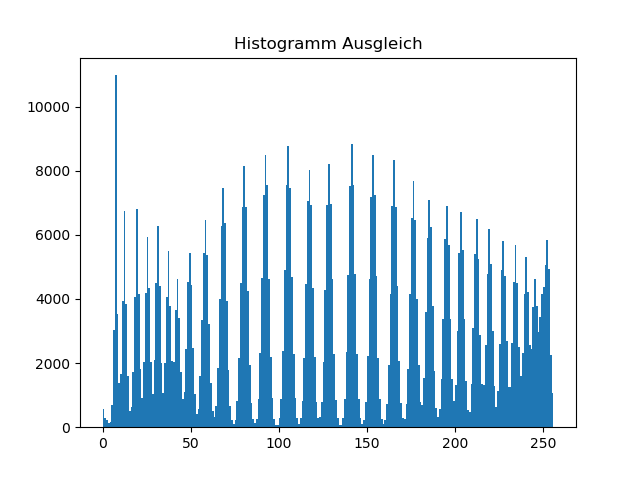
\includegraphics[width=\textwidth]{Sources/Anhang/resize_0250_HA.png}
\end{minipage}
\begin{minipage}{0.49\textwidth}
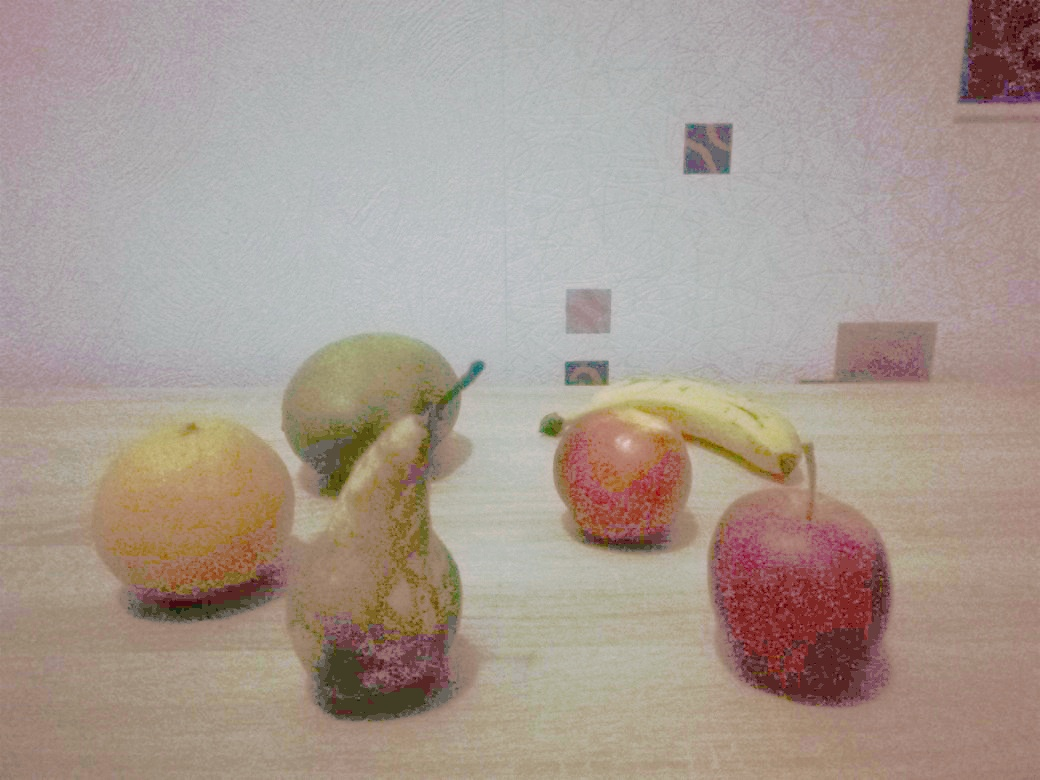
\includegraphics[width=.8\textwidth]{Sources/Anhang/resize_0250_HS.jpg}
\end{minipage}
\begin{minipage}{0.49\textwidth}
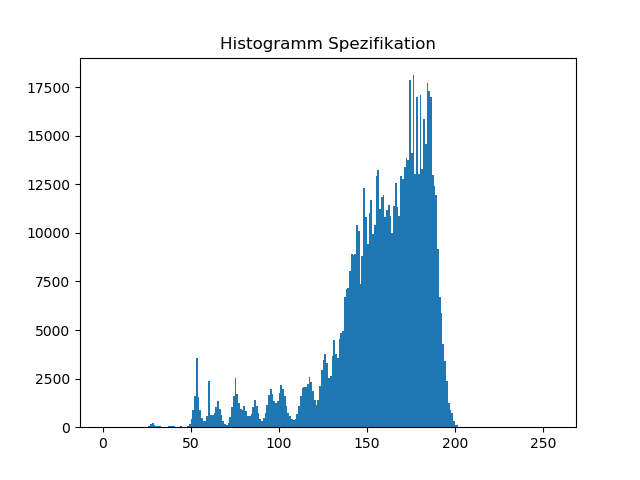
\includegraphics[width=\textwidth]{Sources/Anhang/resize_0250_HS.png}
\end{minipage}
\caption{Helligkeitsverteilung und der Einfluss der Normalisierungs-Algorithmen auf das Testbild}
\label{img:hellver}
\end{figure}

\begin{figure}[htb]
\center
\begin{minipage}{0.19\textwidth}
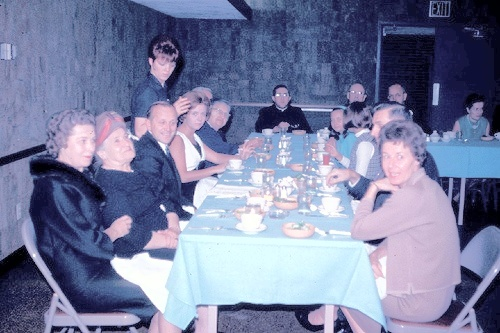
\includegraphics[width=\textwidth]{images/anomalien/HA/000613.jpg}
\end{minipage}
\begin{minipage}{0.19\textwidth}

\includegraphics[width=\textwidth]{images/anomalien/HA/000750.jpg}
\end{minipage}
\begin{minipage}{0.19\textwidth}
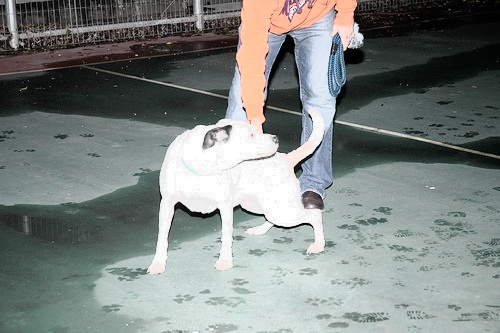
\includegraphics[width=\textwidth]{images/anomalien/HA/000777.jpg}
\end{minipage}
\begin{minipage}{0.19\textwidth}
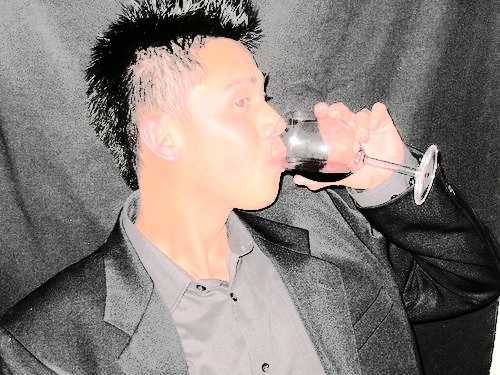
\includegraphics[width=\textwidth]{images/anomalien/HA/001608.jpg}
\end{minipage}
\begin{minipage}{0.19\textwidth}
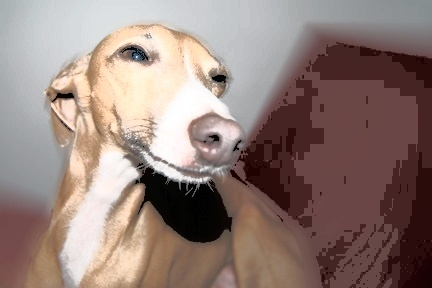
\includegraphics[width=\textwidth]{images/anomalien/HA/003339.jpg}
\end{minipage}
\begin{minipage}{\textwidth}
\hspace{\textwidth}
\end{minipage}
\begin{minipage}{0.19\textwidth}
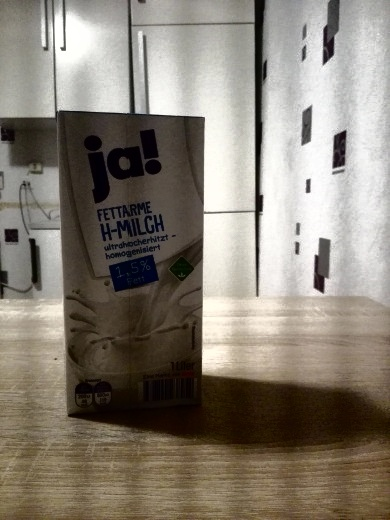
\includegraphics[width=\textwidth]{images/anomalien/HA/image41.jpg}
\end{minipage}
\begin{minipage}{0.19\textwidth}
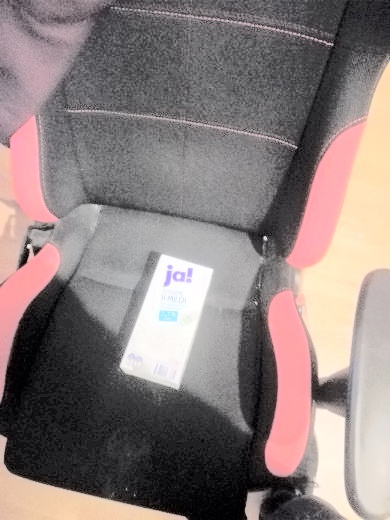
\includegraphics[width=\textwidth]{images/anomalien/HA/image67.jpg}
\end{minipage}
\begin{minipage}{0.19\textwidth}
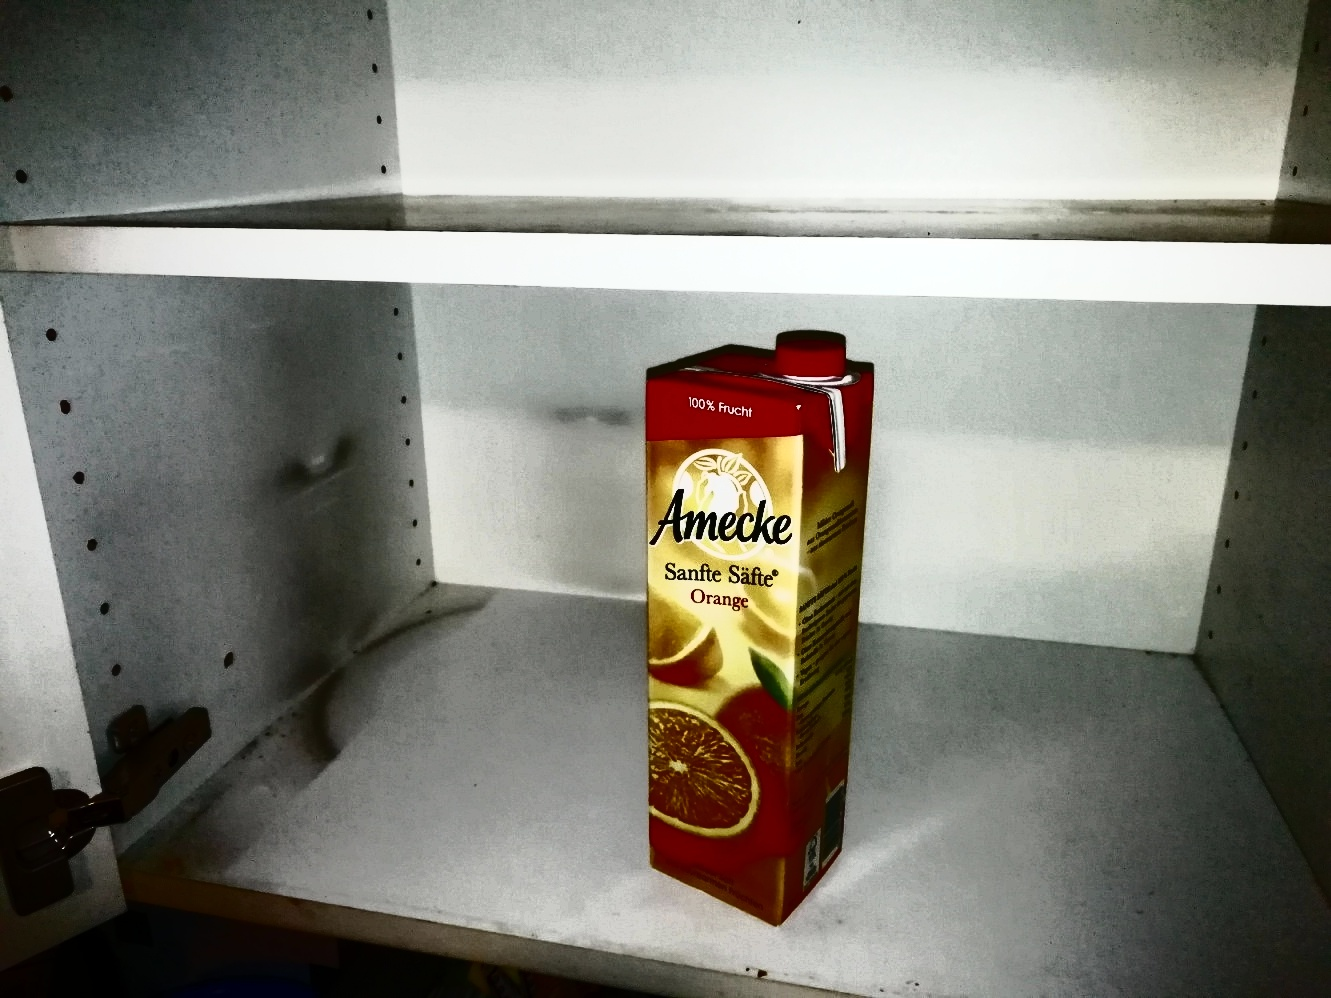
\includegraphics[width=\textwidth]{images/anomalien/HA/image104.jpg}
\end{minipage}
\begin{minipage}{0.19\textwidth}
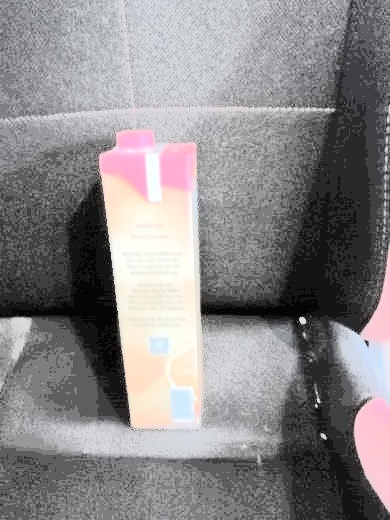
\includegraphics[width=\textwidth]{images/anomalien/HA/image157.jpg}
\end{minipage}
\begin{minipage}{0.19\textwidth}
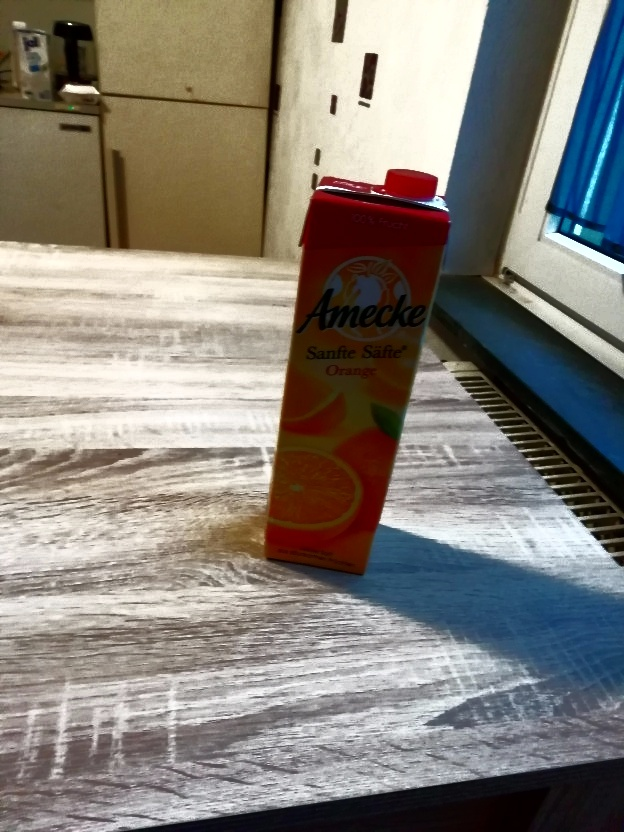
\includegraphics[width=\textwidth]{images/anomalien/HA/IMG_20181209_160502.jpg}
\end{minipage}
\begin{minipage}{\textwidth}
\hspace{\textwidth}
\end{minipage}
\begin{minipage}{0.19\textwidth}
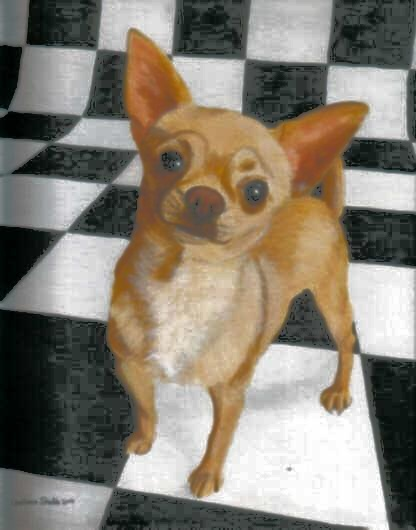
\includegraphics[width=\textwidth]{images/anomalien/HA/n02085620_952.jpg}
\end{minipage}
\begin{minipage}{0.19\textwidth}
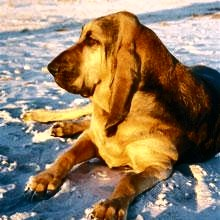
\includegraphics[width=.8\textwidth]{images/anomalien/HA/n02088466_9359.jpg}
\end{minipage}
\begin{minipage}{0.19\textwidth}
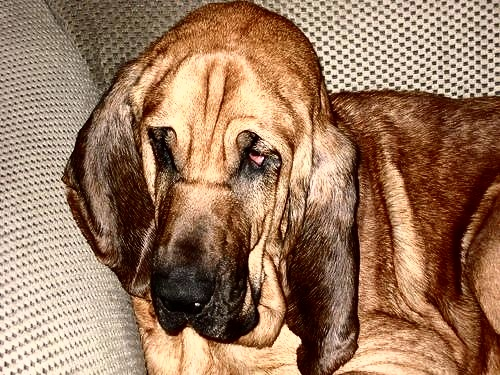
\includegraphics[width=\textwidth]{images/anomalien/HA/n02088466_9691.jpg}
\end{minipage}
\begin{minipage}{0.19\textwidth}
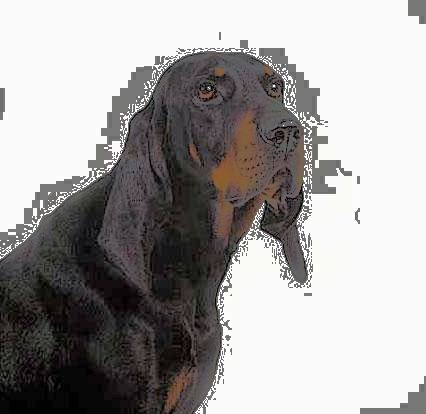
\includegraphics[width=\textwidth]{images/anomalien/HA/n02089078_4544.jpg}
\end{minipage}
\begin{minipage}{0.19\textwidth}
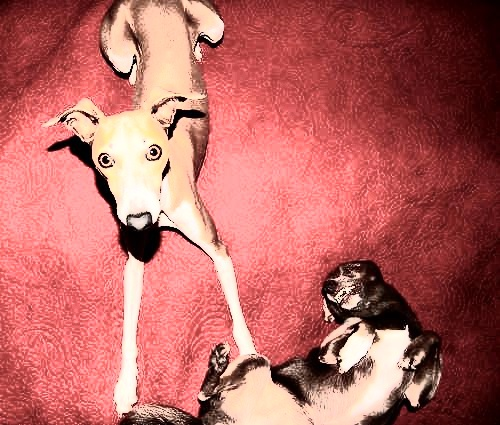
\includegraphics[width=\textwidth]{images/anomalien/HA/n02091032_12113.jpg}
\end{minipage}
\caption{Auftretende Farbanomalien in den drei Datensätzen durch den Histogramm-Ausgleich. Oben: PascalVOC-Datensatz, Mitte: Nahrungsmittel-Datensatz, Unten: Stanford Dog-Datensatz}
\label{img:anoHA}
\end{figure}

\begin{figure}[htb]
\center
\begin{minipage}{0.19\textwidth}
\includegraphics[width=\textwidth]{images/anomalien/HS/007911.jpg}
\end{minipage}
\begin{minipage}{0.19\textwidth}
\includegraphics[width=\textwidth]{images/anomalien/HS/007935.jpg}
\end{minipage}
\begin{minipage}{0.19\textwidth}
\includegraphics[width=\textwidth]{images/anomalien/HS/008085.jpg}
\end{minipage}
\begin{minipage}{0.19\textwidth}
\includegraphics[width=\textwidth]{images/anomalien/HS/008103.jpg}
\end{minipage}
\begin{minipage}{0.19\textwidth}
\includegraphics[width=\textwidth]{images/anomalien/HS/008112.jpg}
\end{minipage}
\begin{minipage}{\textwidth}
\hspace{\textwidth}
\end{minipage}
\begin{minipage}{0.19\textwidth}
\includegraphics[width=\textwidth]{images/anomalien/HS/image157.jpg}
\end{minipage}
\begin{minipage}{0.19\textwidth}
\includegraphics[width=\textwidth]{images/anomalien/HS/image159.jpg}
\end{minipage}
\begin{minipage}{0.19\textwidth}
\includegraphics[width=\textwidth]{images/anomalien/HS/image160.jpg}
\end{minipage}
\begin{minipage}{0.19\textwidth}
\includegraphics[width=\textwidth]{images/anomalien/HS/image240.jpg}
\end{minipage}
\begin{minipage}{0.19\textwidth}
\includegraphics[width=\textwidth]{images/anomalien/HS/IMG_20181209_160802.jpg}
\end{minipage}
\begin{minipage}{\textwidth}
\hspace{\textwidth}
\end{minipage}
\begin{minipage}{0.19\textwidth}
\includegraphics[width=\textwidth]{images/anomalien/HS/n02085620_1620.jpg}
\end{minipage}
\begin{minipage}{0.19\textwidth}
\includegraphics[width=.8\textwidth]{images/anomalien/HS/n02085620_2188.jpg}
\end{minipage}
\begin{minipage}{0.19\textwidth}
\includegraphics[width=\textwidth]{images/anomalien/HS/n02085782_1503.jpg}
\end{minipage}
\begin{minipage}{0.19\textwidth}
\includegraphics[width=\textwidth]{images/anomalien/HS/n02085782_1626.jpg}
\end{minipage}
\begin{minipage}{0.19\textwidth}
\includegraphics[width=\textwidth]{images/anomalien/HS/n02088094_1406.jpg}
\end{minipage}
\caption{Auftretende Farbanomalien in den drei Datensätzen durch die Histogramm-Spezifikation. Oben: PascalVOC-Datensatz, Mitte: Nahrungsmittel-Datensatz, Unten: Stanford Dog-Datensatz}
\label{img:anoHS}
\end{figure}


\end{appendices}